\section{use cases}

\subsection{Chatbot platform}
We decided to build chatbot through Facebook, which has more than 2 billion users until 2017. Facebook Messenger can provide an intensively tested and user-friendly interface because many people are already using it. In addition, users who are using Facebook do not require a separate download, so we can meet Requirements A4.

\subsection{Description of practical usage}

\begin{figure}[htbp]
\centerline{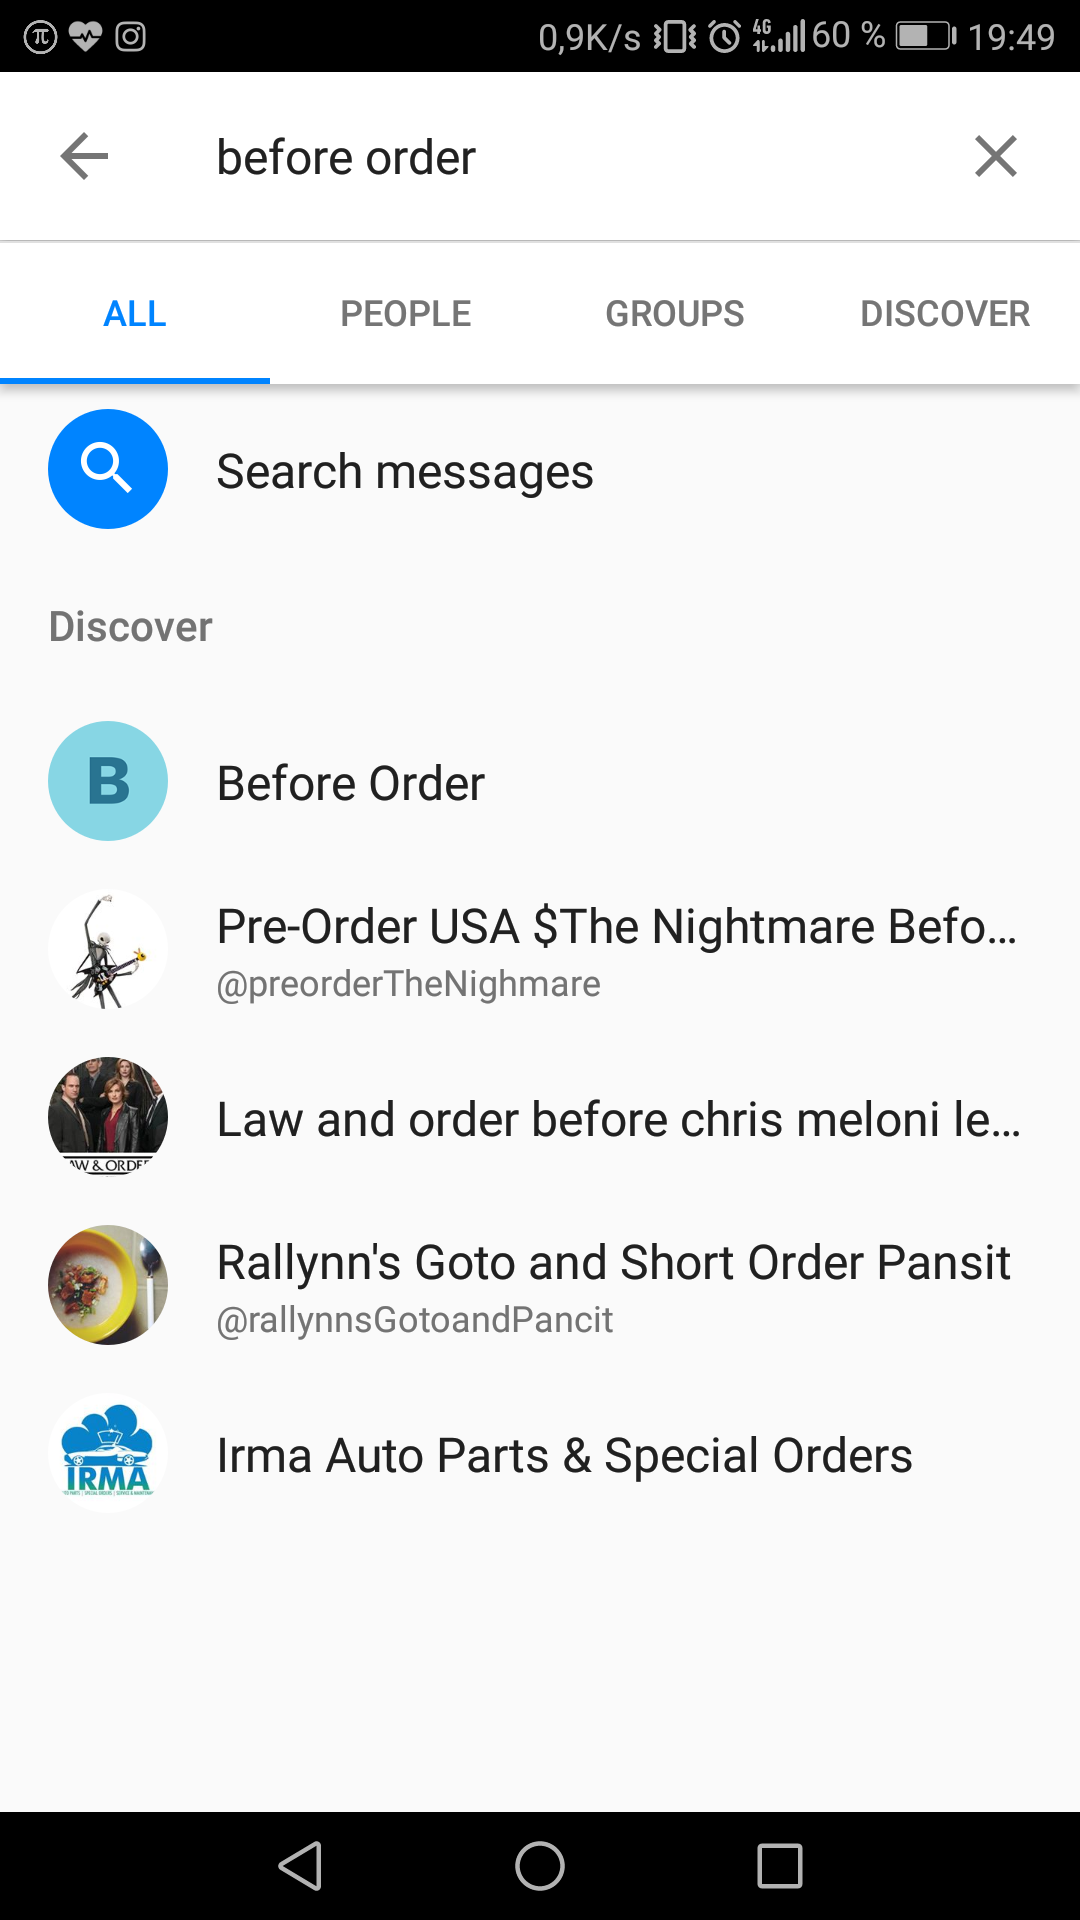
\includegraphics[height=\custompicheight]{./pictures/Screenshot_20181125-194915}}
\caption{Search \emph{Before Order} in Facebook Messenger}
\label{fig:Before Order_search}
\end{figure}
\FloatBarrier
\subsubsection{Search Before Order}
Access Facebook Messenger through a variety of devices. Then users should search our chatbot ‘Before Order’ in Facebook Messenger. As seen from the above capture, ‘Before Order’ is available on smartphone and therefore this meets the requirement A.1.

\begin{figure}[htbp]
\centerline{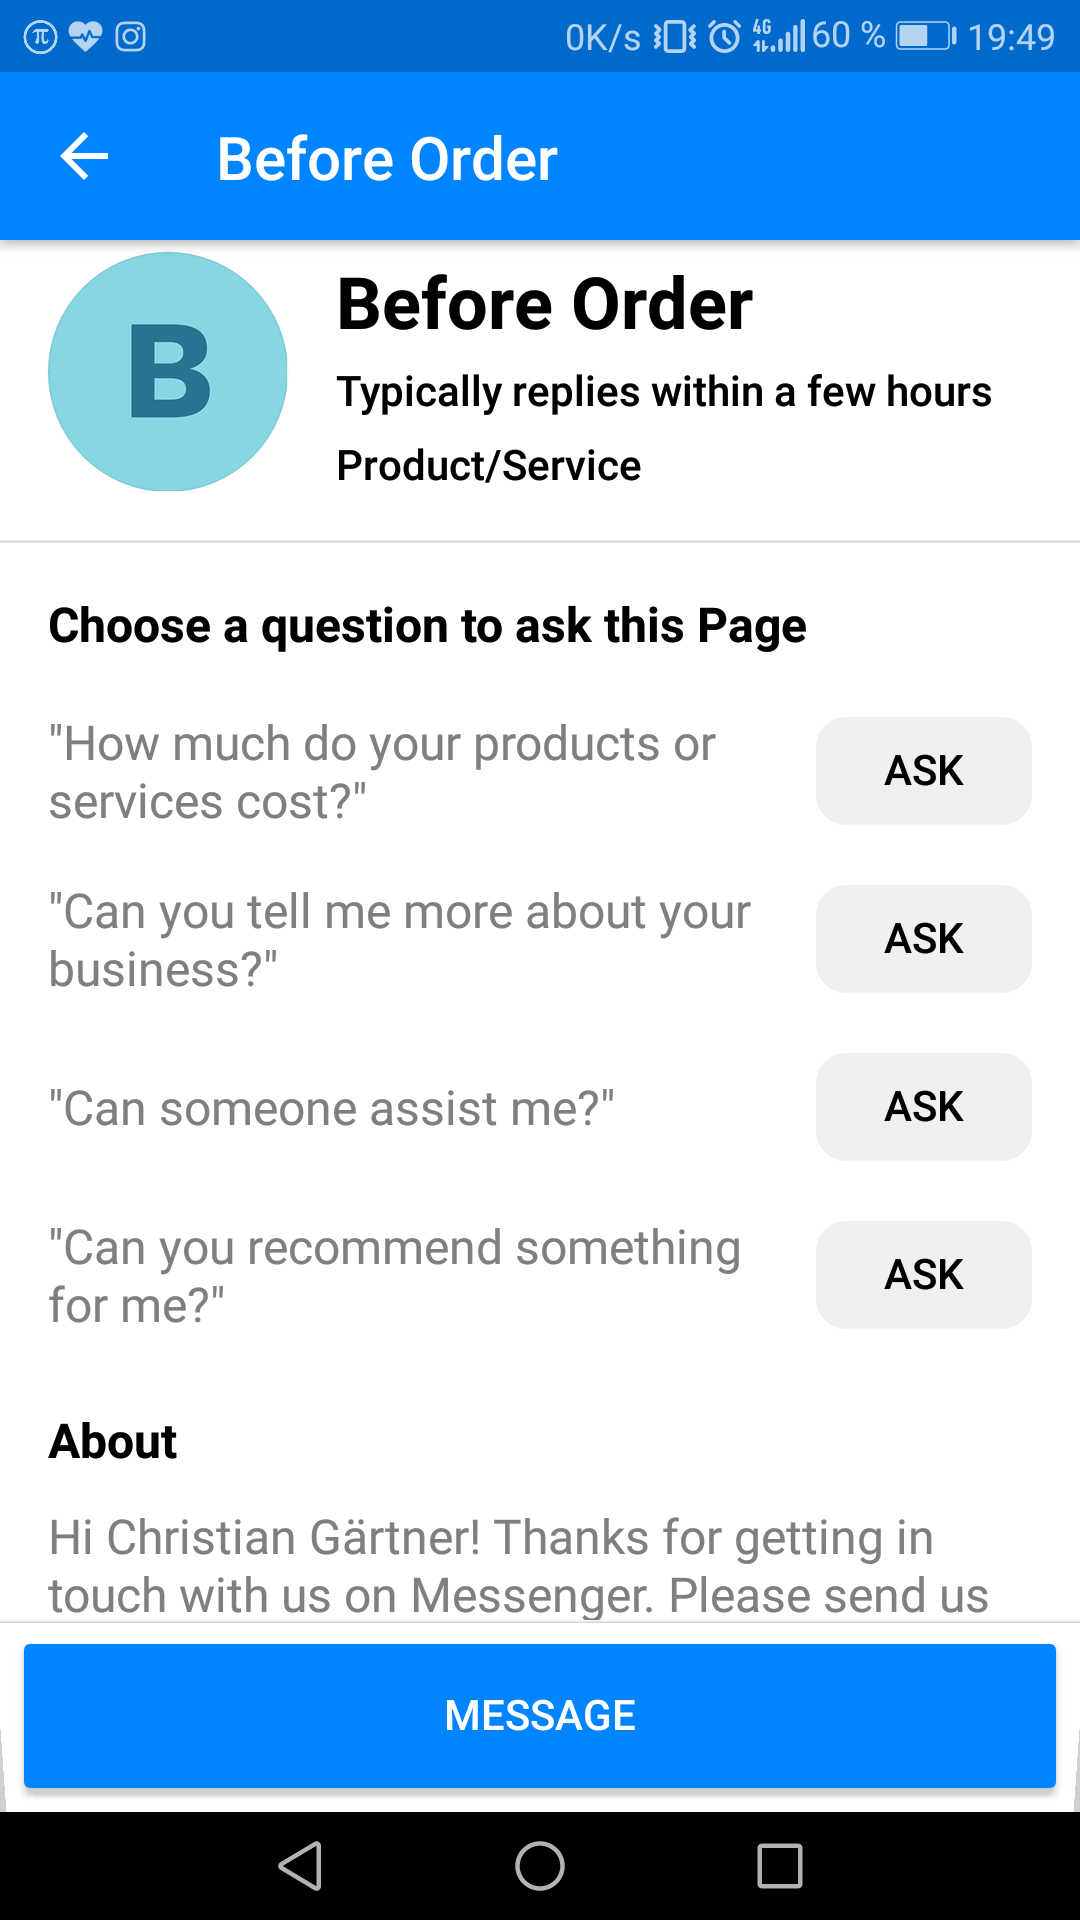
\includegraphics[height=\custompicheight]{./pictures/Screenshot_20181125-194938}}
\caption{Initial screen page of \emph{Before Order}}
\label{fig:Before Order_initial_screen}
\end{figure}
\FloatBarrier
\subsubsection{Start messaging}
 If users find ‘Before Order’, they can click it and start Messenger chatting. Click the button ‘Message’ or ‘시작하기’ in order to send messages to chatbot. By using existing Facebook Messenger, ‘Before Order’ is easily accessible to billions of people using Facebook and its Messenger. Users even do not need to newly sign up for ‘Before Order’.


\begin{figure}[htbp]
\centerline{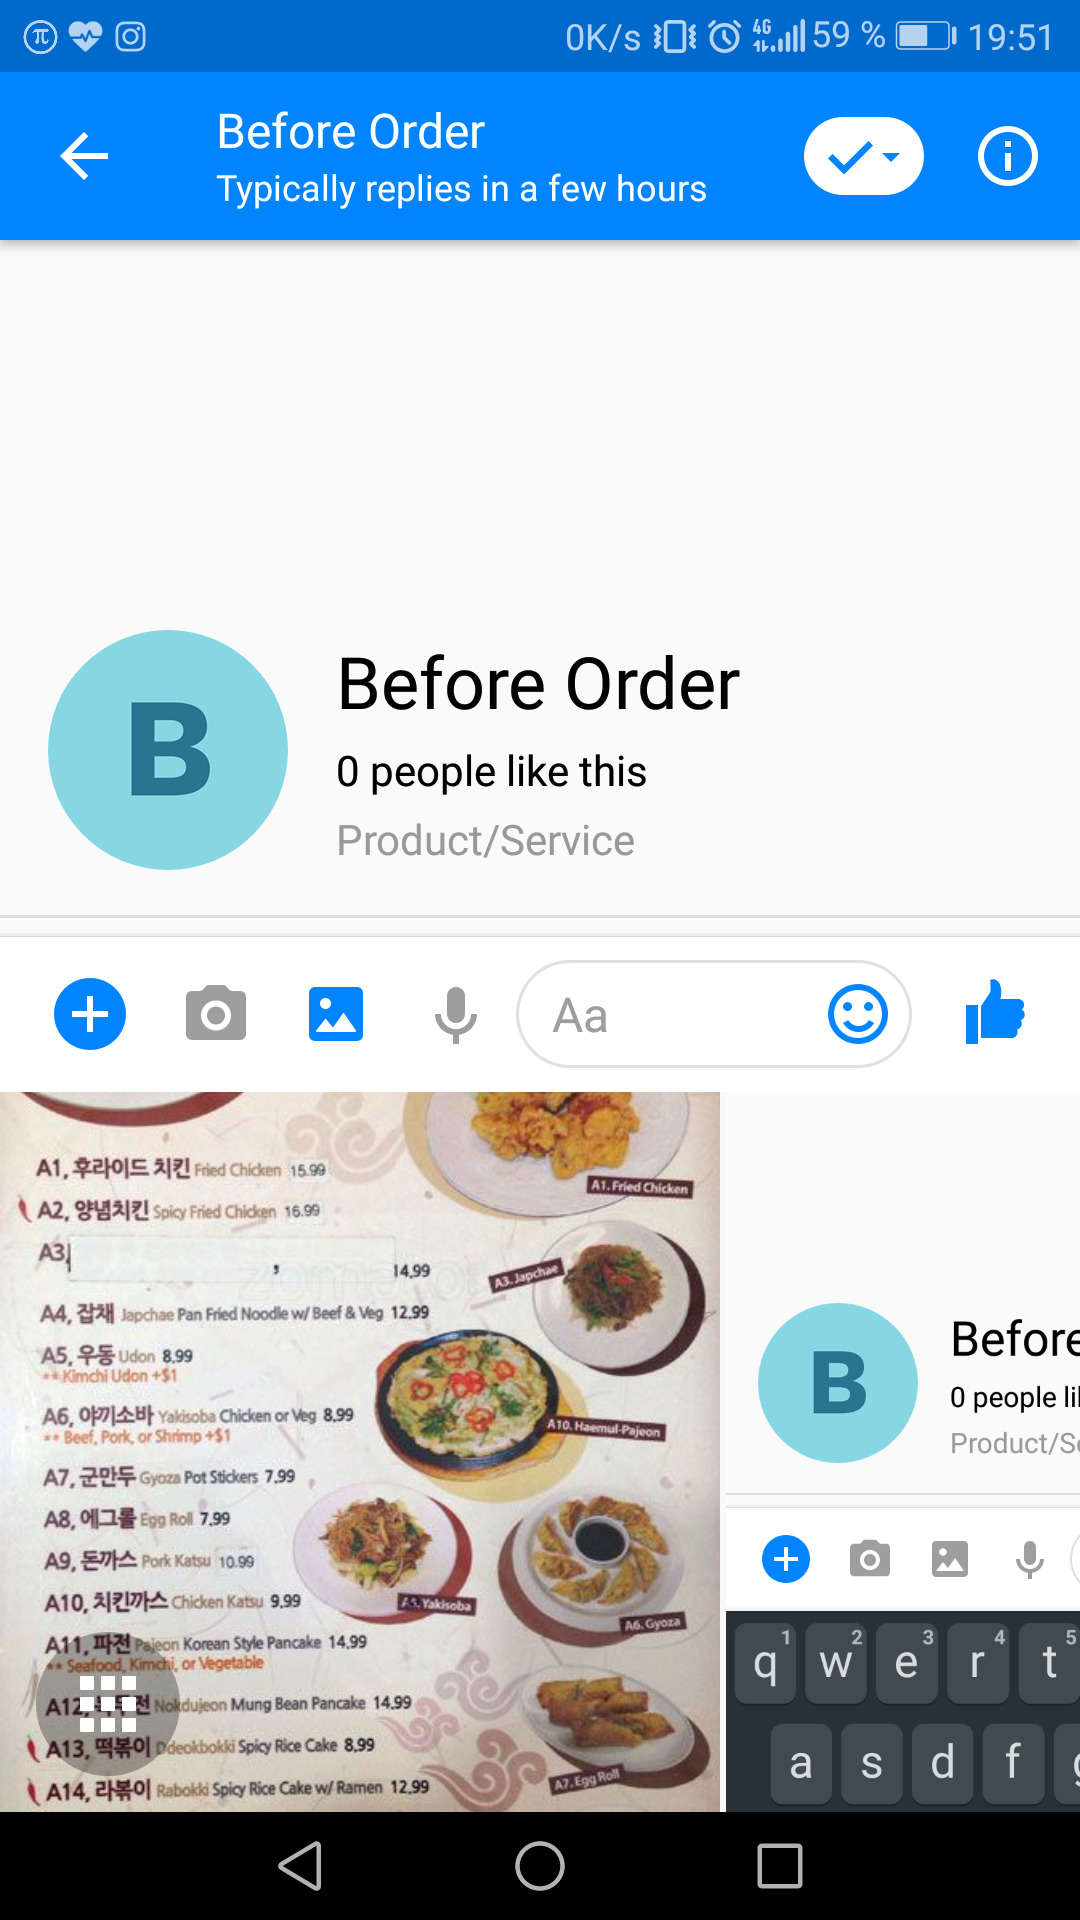
\includegraphics[height=\custompicheight]{./pictures/Screenshot_20181125-195124}}
\caption{Selecting menu picture as an input}
\label{fig:Before Order_input_selection}
\end{figure}
\FloatBarrier
\subsubsection{Select input}
 If users entered ‘Before Order’ page, the chatbot will deliver a brief greeting. Our chatbot was made for foreigners who had trouble translating the Korean menu. Therefore ‘Before Order’ take optimized way of relieving their inconvenience. Whenever users find it difficult to interpret the Korean menu in a restaurant, they can just take a picture of the menu and then select the picture to send.


\begin{figure}[htbp]
\centerline{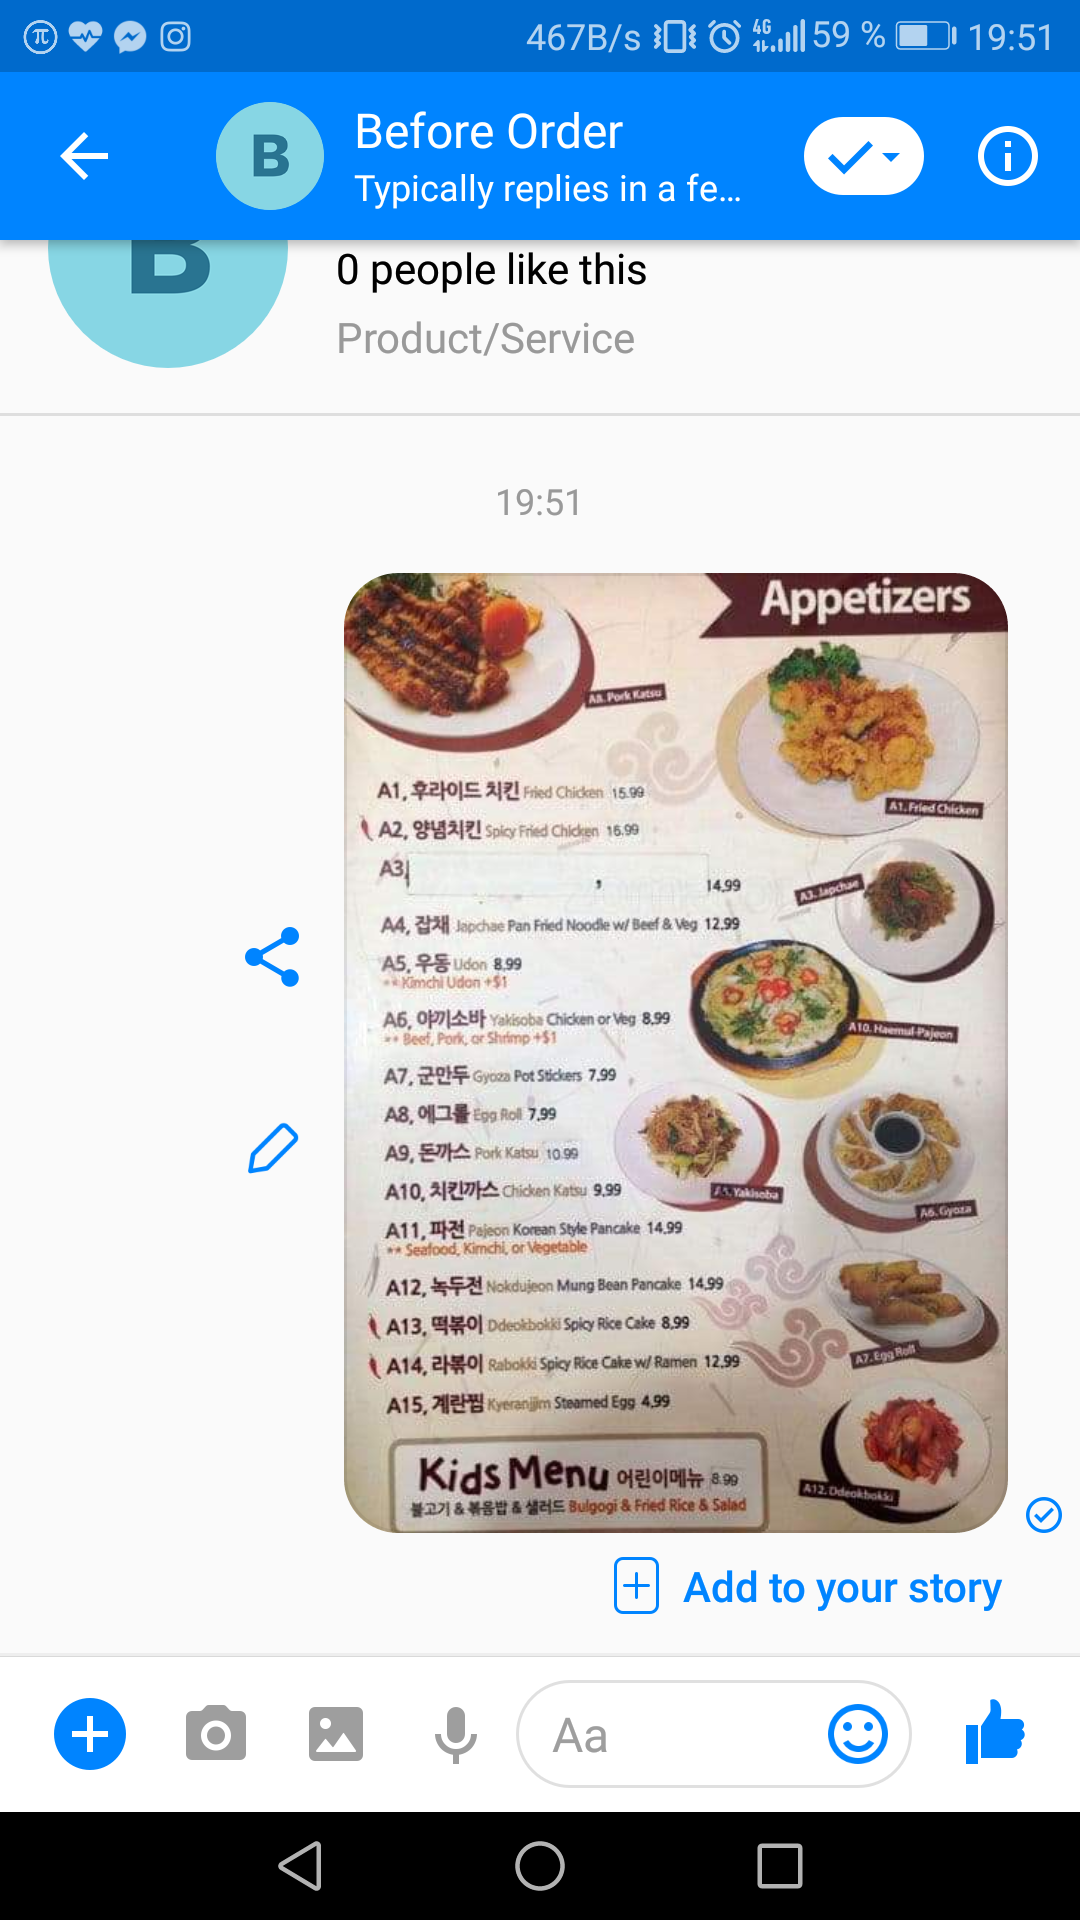
\includegraphics[height=\custompicheight]{./pictures/Screenshot_20181125-195145}}
\caption{Users sending input to \emph{Before Order}}
\label{fig:Before Order_send_Input}
\end{figure}
\FloatBarrier
\subsubsection{Send input}
The users who are not familiar with Korean menus can get the information they want through 'before order'. Users take a picture of the menu using the camera on the device you are carrying. Using Facebook Messenger, the users can send a message through camera or photo button in the lower left corner. Then send 'before order' and we will begin to recognize the menu.


\begin{figure}[htbp]
\centerline{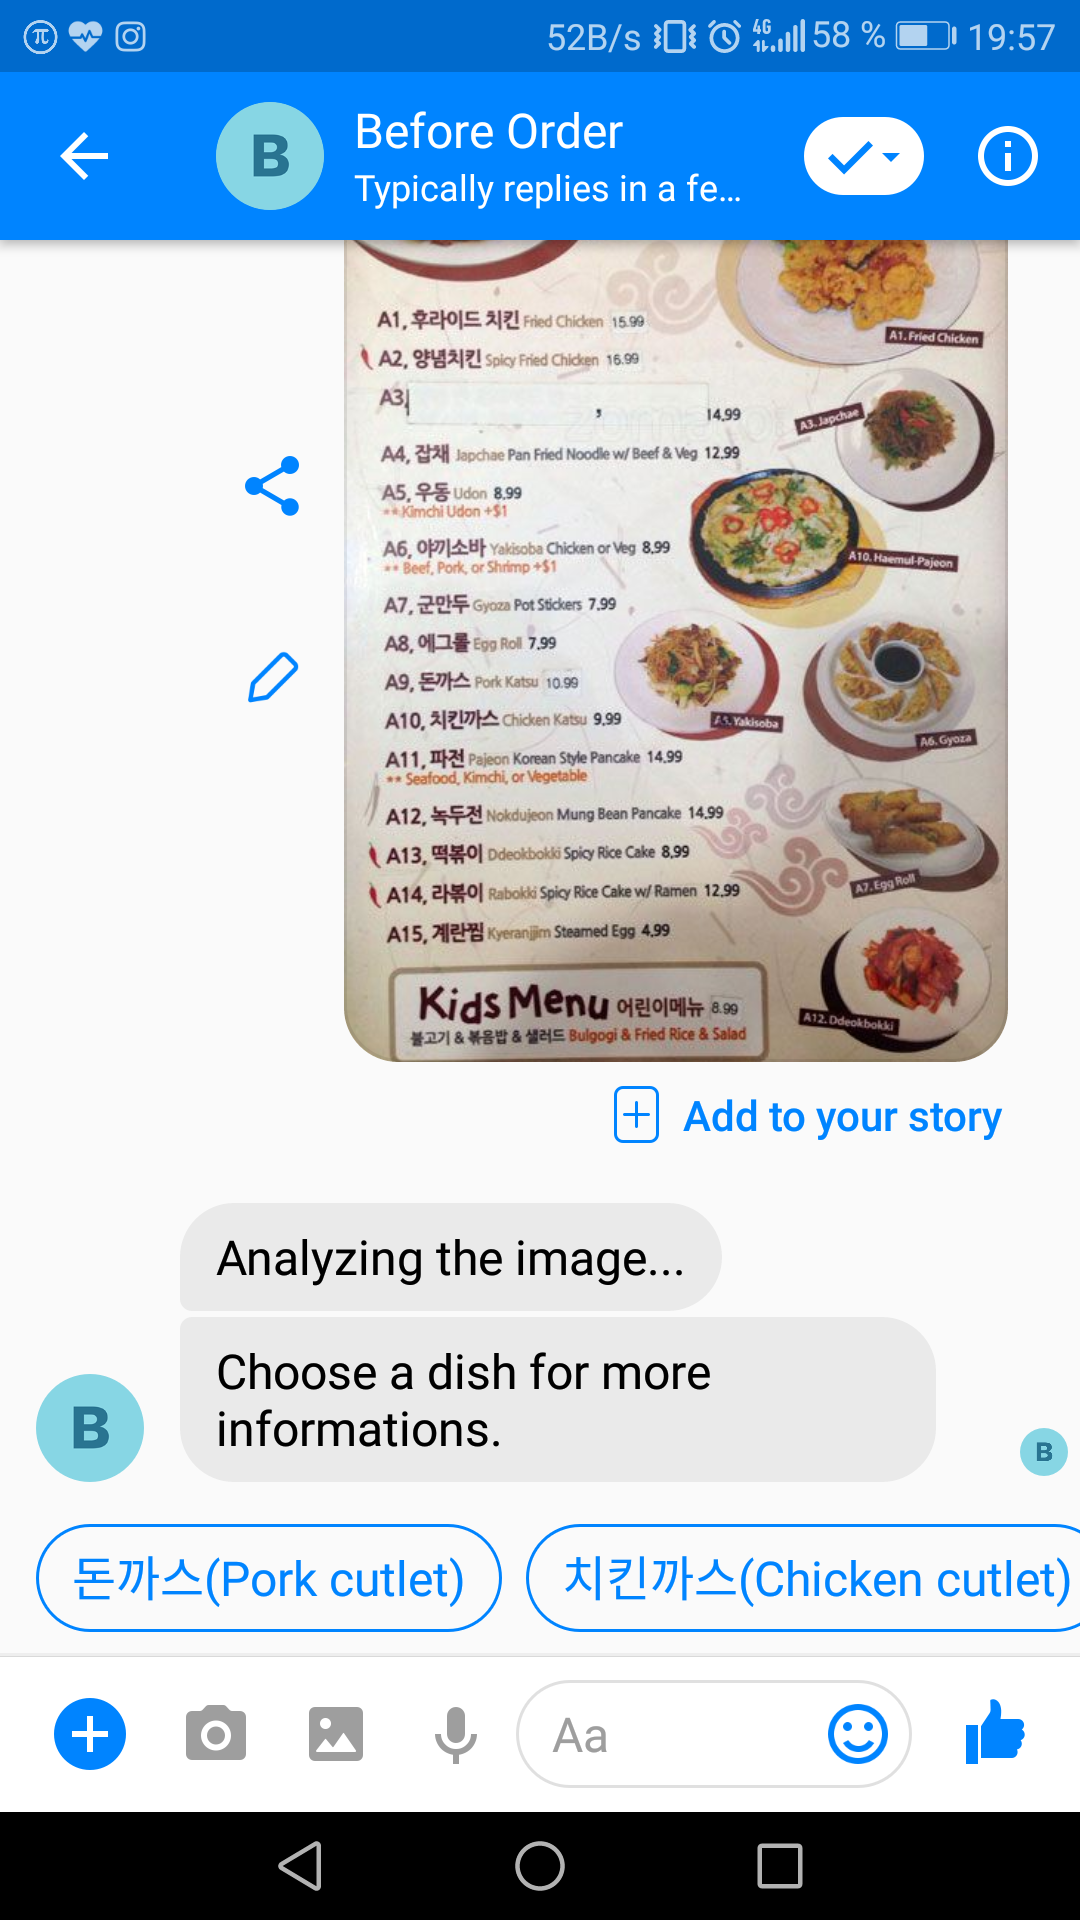
\includegraphics[height=\custompicheight]{./pictures/Screenshot_20181125-195722}}
\caption{Analyzing the input sent from user}
\label{fig:Before Order_analyze_input}
\end{figure}
\FloatBarrier
\subsubsection{Wait for the result}
 Based on the pictures sent by the user, we will begin to analyze the images. Users can view the message 'Analyzing the image' while the image is being analyzed and may be asked to select the desired information after the analysis is completed. Users can click on a list of buttons that are created based on the text we recognize.


\begin{figure}[htbp]
\centerline{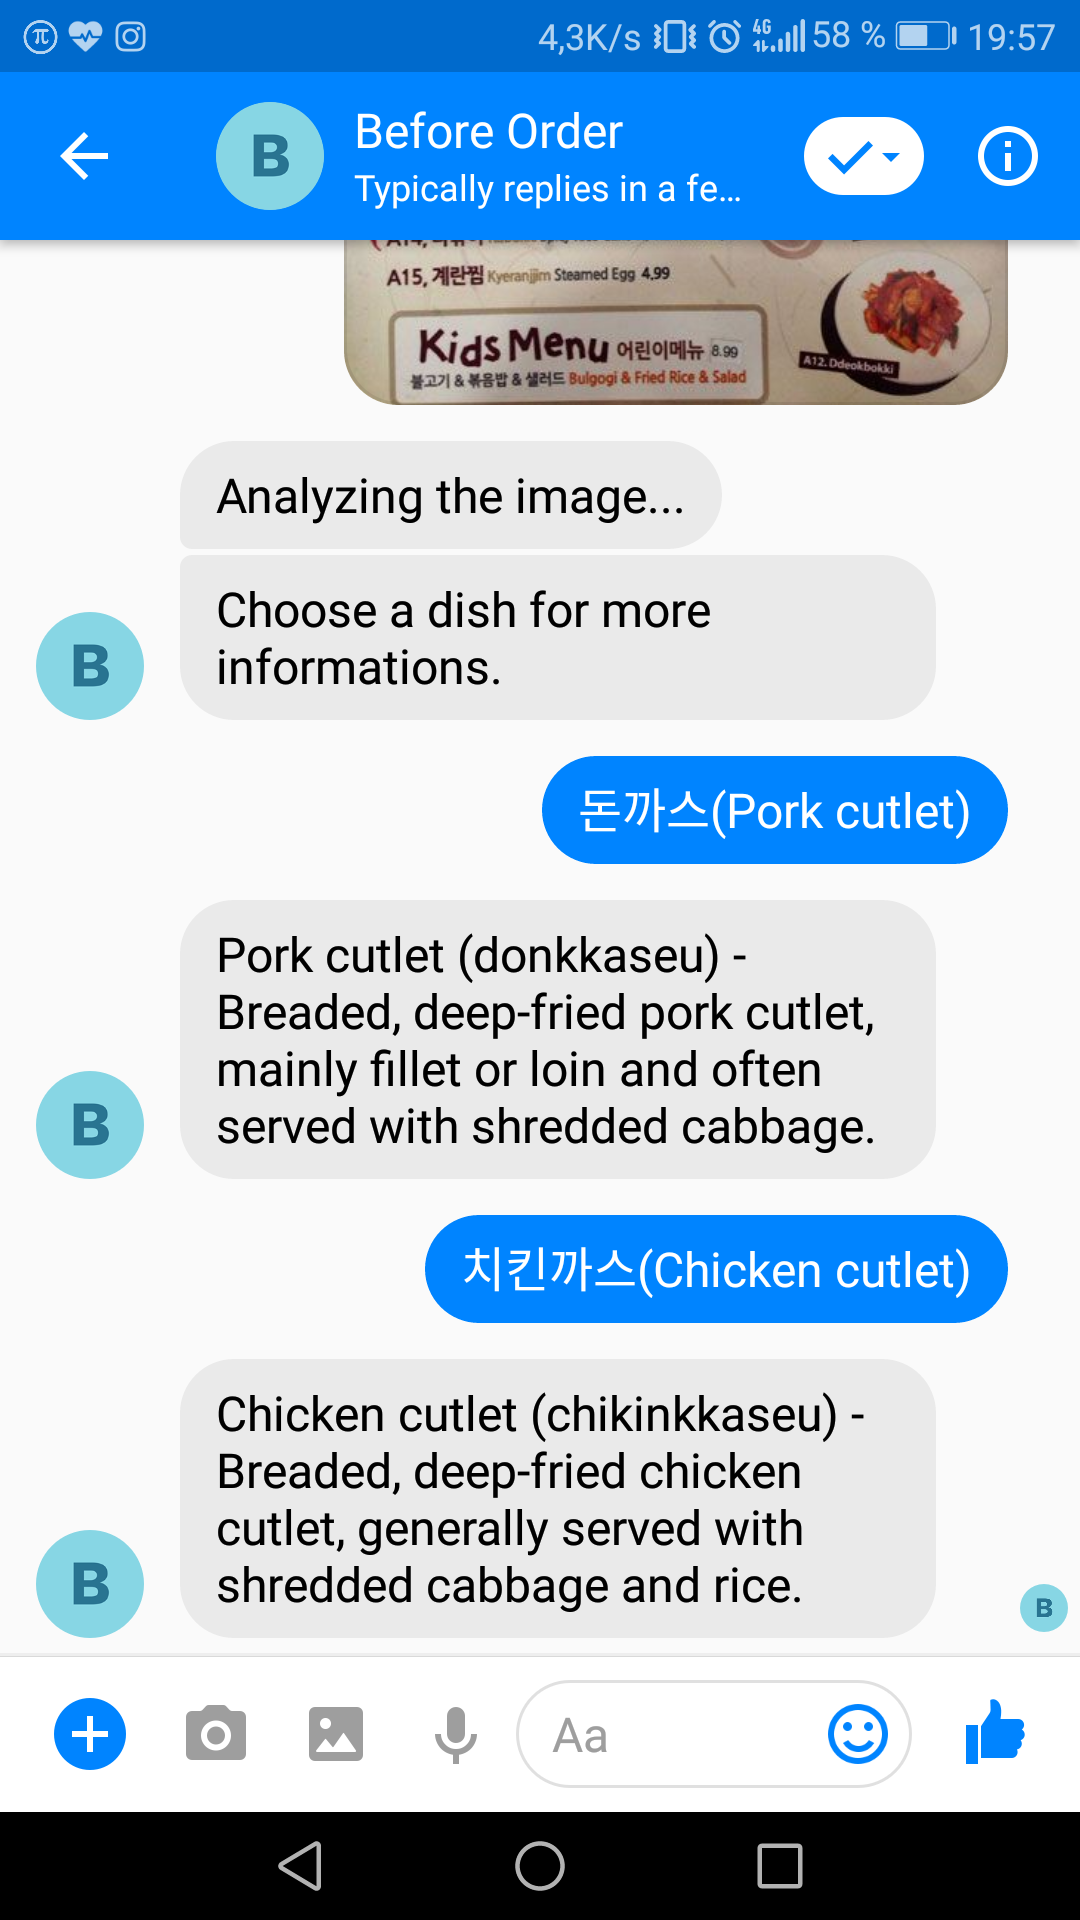
\includegraphics[height=\custompicheight]{./pictures/Screenshot_20181125-195753}}
\caption{Showing information about the selected dish}
\label{fig:Before Order_show_dish information}
\end{figure}
\FloatBarrier
\subsubsection{Receive a selected dish information}
When users click the button with dish name, dish information appears in the way as the picture above. As stated in the requirement A.8, All information is provided in English except for user input. As a result of chatting with ‘Before Order’, users get a brief description of the dish and information about its ingredients. This is a key feature of ‘Before Order’ which satisfied the requirement A.9. To provide information from the database with such reliability, one more thing – price value should be taken into consideration. Though dish name ‘치킨가스’ is displayed along with the price value 9.99 in the given menu picture, ‘Before Order’ succeeded in recognizing only the dish name by adding the function of excluding the price portion. These features make it possible to retrieve the right information from the database and therefore meet the requirement A.12. To follow the requirement A.13, all the dish information was taken form Wikipedia and this guarantee both accuracy and reliability. Small but important feature is the Romanization. Inside the parentheses, there is Korean dish name written in Roman characters like ‘donkkaseu’ and ‘chikinkkaseu’. By referring to the Romanization, users can well pronounce Korean dish name in the case of ordering food .This function is implemented to meet second condition inside the requirement A.13.


\subsection{Addressing error-prone cases}

\begin{figure}[htbp]
\centerline{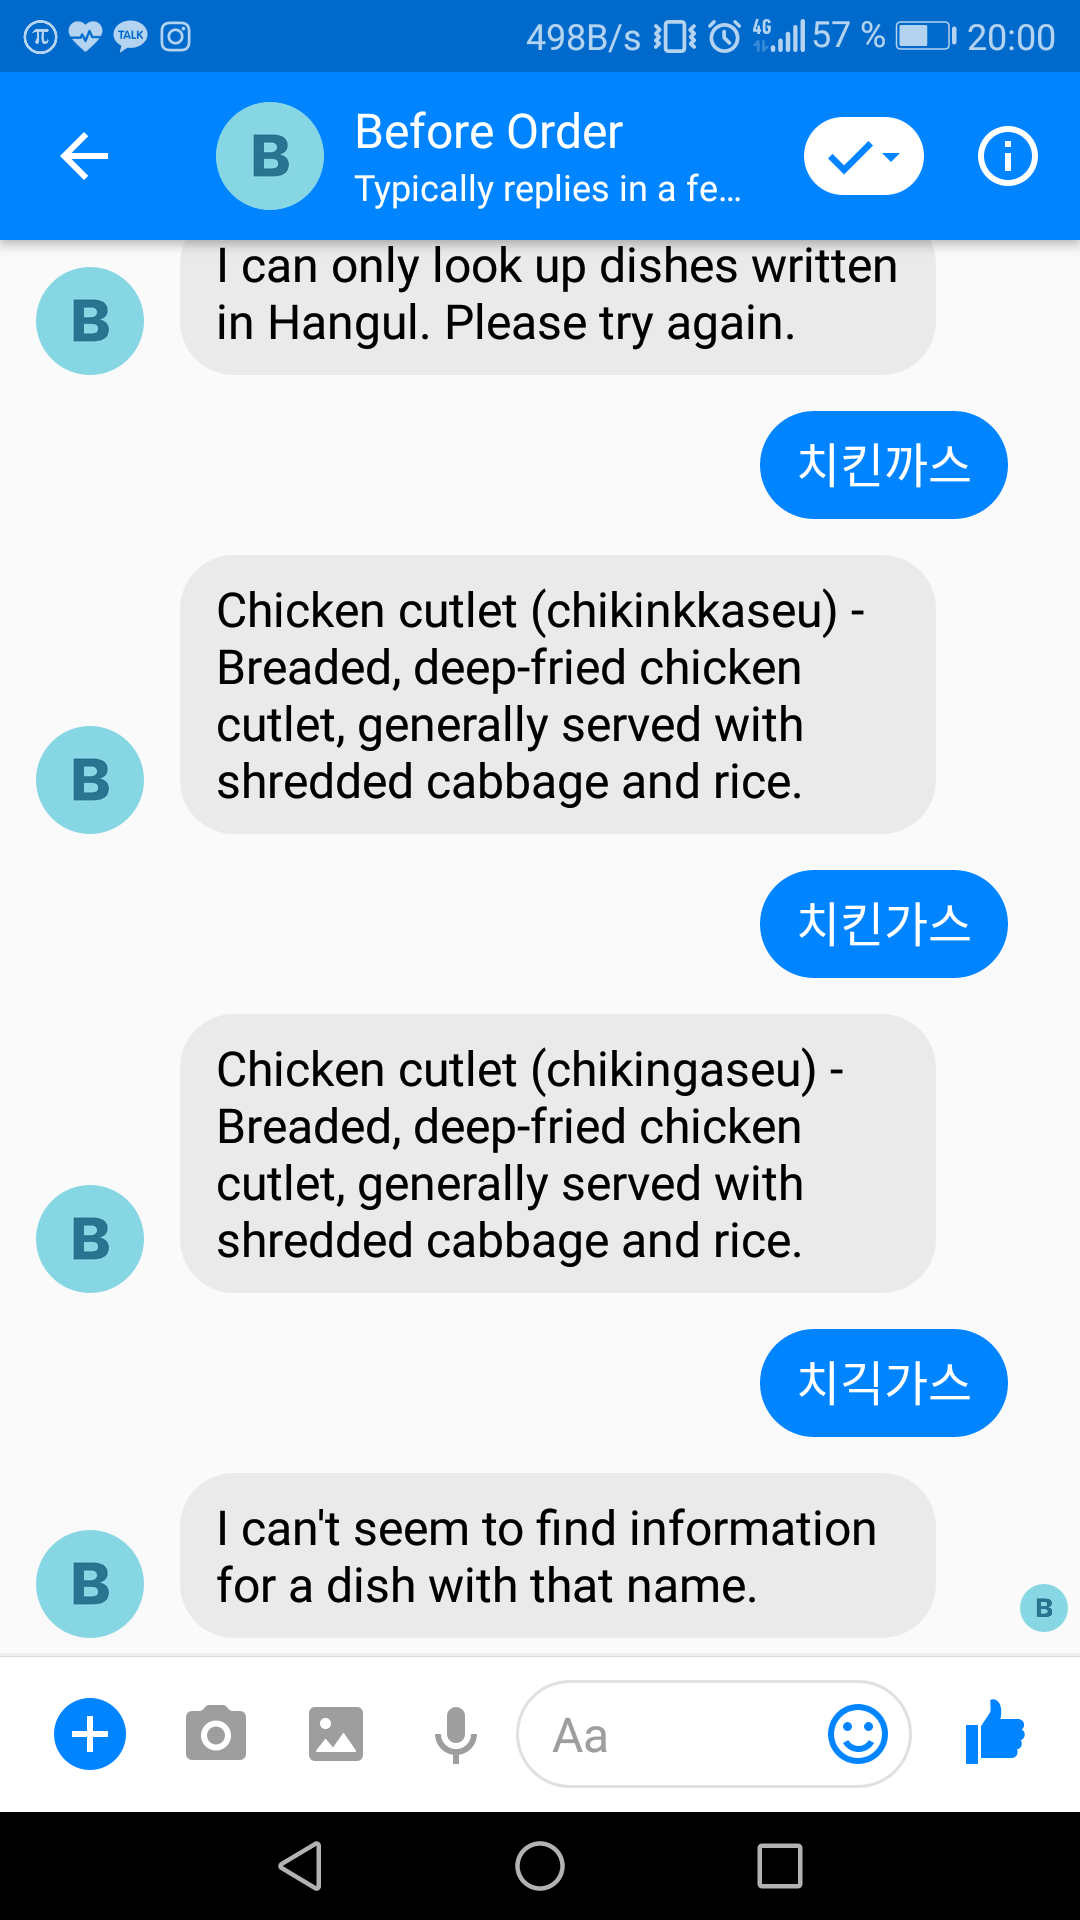
\includegraphics[height=\custompicheight]{./pictures/Screenshot_20181125-200020}}
\caption{Handling various error-prone cases}
\label{fig:Before Order_features}
\end{figure}
\FloatBarrier
The basic function set of ‘Before Order’ is to receive photos sent by users, analyze them, and provide a list of buttons. However as stated in the requirement A.7 and A.10, our chatbot ‘Before Order’ can recognize not only pictures but also Korean inputs – food written in Korean sent by users. Even if the user enters Korean words ‘치킨까스’ or ‘치킨가스’ without menu pictures, It is also able to provide accurate food information. This satisfies the third item of requirement A.13. Furthermore ‘Before Order’ is designed to support various expressions of Hangul. It successfully recognize two different expressions ‘치킨까스’ and ‘치킨가스’ as the same word. At the same time, ‘Before Order’ can also distinguish between dish names and random letter clusters. For random letter clusters like ‘치긱가스’, the chatbot send a response ‘I can’t seem to find the information for a dish with that name.’ - notifying something is wrong. This meets the requirement A.11.

\subsection{Handling inappropriate input format}

\begin{figure}[htbp]
\centerline{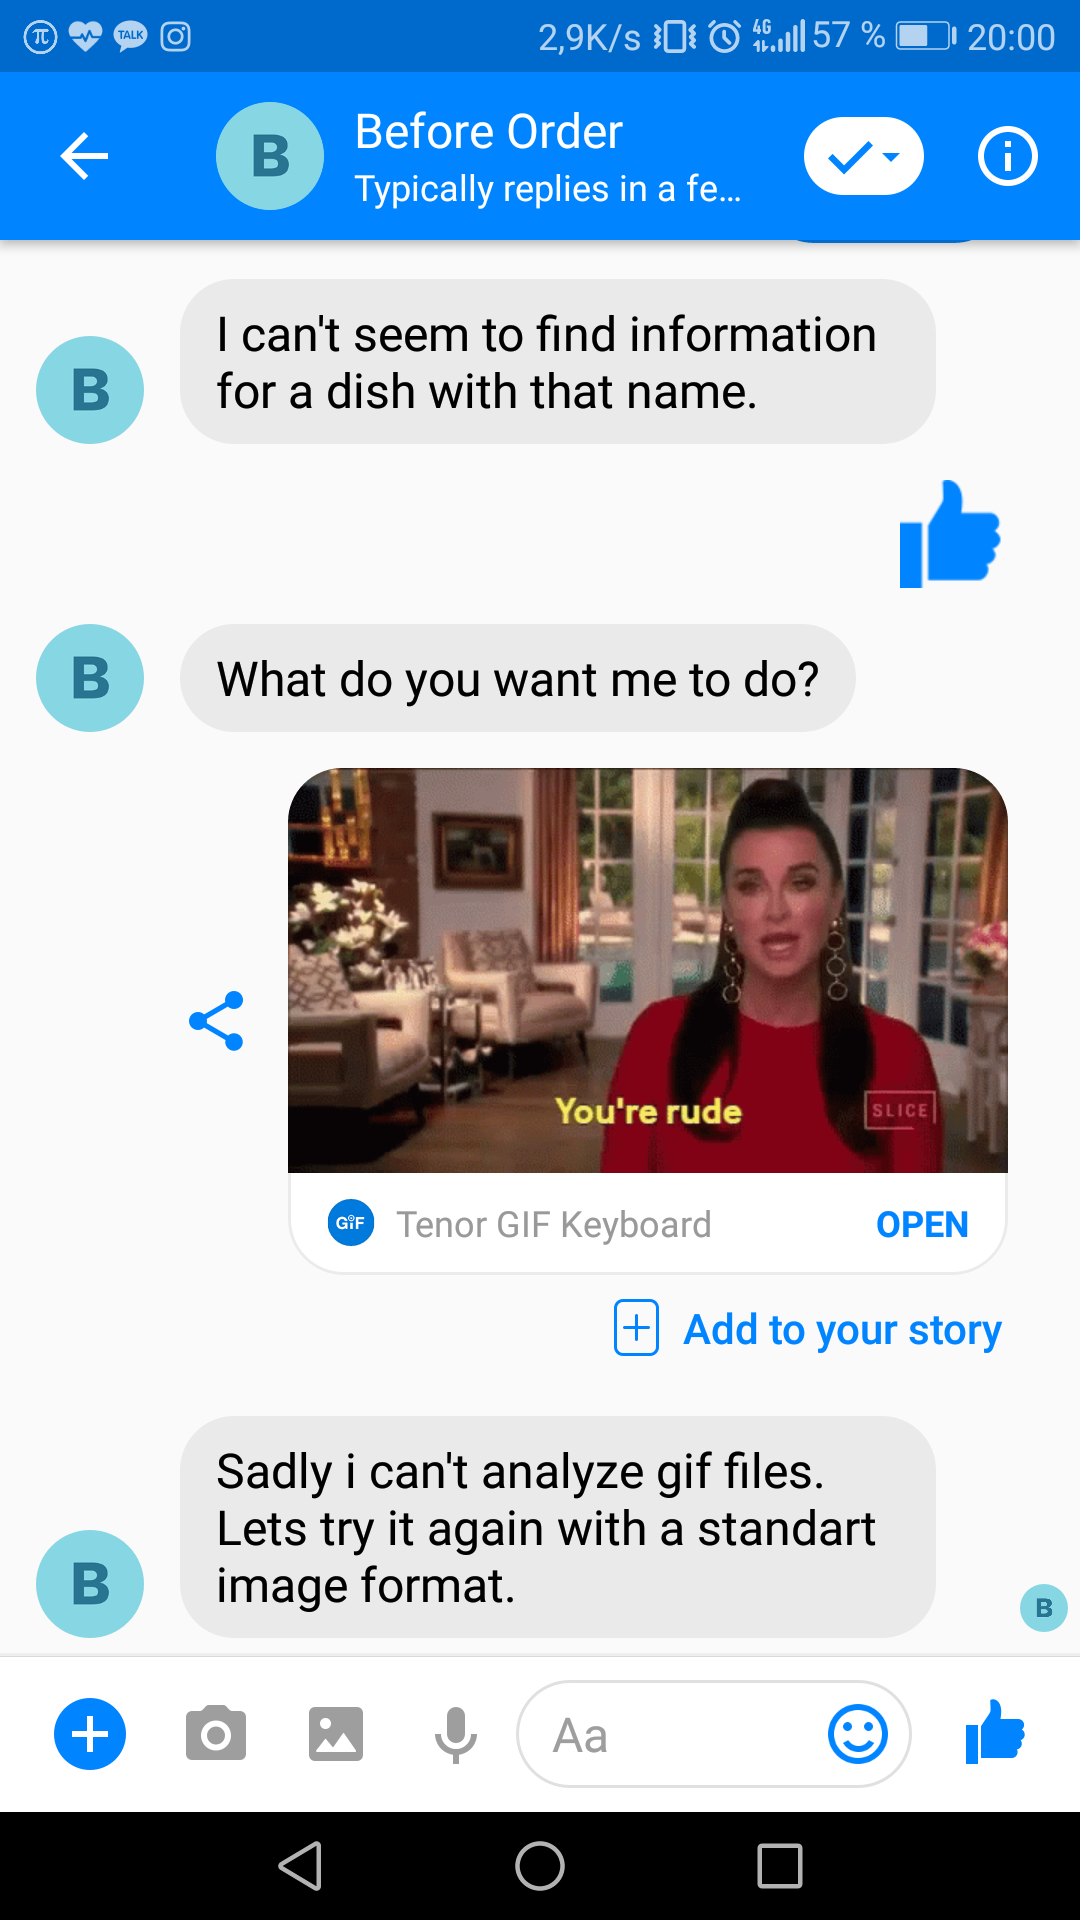
\includegraphics[height=\custompicheight]{./pictures/Screenshot_20181125-200053}}
\caption{Handling inappropriate image format}
\label{fig:Before Order_handling_error}
\end{figure}
\FloatBarrier

Just like the case of random letter clusters ‘치긱가스’, ‘Before Order’ can distinguish between right and wrong. If the user sends pictures in invalid format or pictures without a menu, the chatbot recognize them and give an appropriate response depending on the situation. This series of actions is designed to meet requirement A.11.


\subsection{Key functions}
As stated in Requirements A.6, we reduce the process of users searching menus in English and retrieving information about the word again. The users take pictures and send them to us without having to search again. Also, when users open the messenger window again, they can always see it again because they have a history of previous messages.

\subsection{Service management}
If the users are using the 'Before Order' and we cannot be aware of the message sent by the user, or if there is something we need to correct it, the users can contact us through the Facebook page. When a user posts a post on our page or sends an developer’s e-mail, we can provide feedback, like a requirement A5. And at the beginning of the conversation, we're specifying a message that we want users to send an email if they need help or if an error is detected.











